\documentclass[A4]{article}

\usepackage[english]{babel}
\usepackage[utf8]{inputenc}
\usepackage{amsmath}
\usepackage{graphicx}
\usepackage{float}
\usepackage{enumitem}
\usepackage[toc,page]{appendix}
\usepackage{url}

\usepackage{geometry}
\geometry{
a4paper,
left=20mm,
top=20mm,
}

\title{Deep Learning Lab2 Report}

\author{Chien-Hsun, Lai}

\date{\today}

\makeatletter
% we use \prefix@<level> only if it is defined
\renewcommand{\@seccntformat}[1]{%
  \ifcsname prefix@#1\endcsname
    \csname prefix@#1\endcsname
  \else
    \csname the#1\endcsname\quad
  \fi}
% define \prefix@section
\newcommand\prefix@section{\thesection. }
\makeatother

\renewcommand{\thesubsection}{\alph{subsection}.}
\begin{document}
\maketitle

\section{Introduction}
In this lab, we'll go through 4 experiments about Deep Image Prior.
To see if a un-trained neural network can learn the intrinsic feature about target image.
We conduct the following experiments:
\begin{itemize}
	\item {First, we'll investigate the influence of different input.
	There are number of inputs. Some of them looks like the target image.
	Some of them are completely random noise.
	To see how each input converges.}
	\item {Second, we'll do blind denoising. To check if the network can learn the pattern first. Then it learns the noise.}
	\item {Third, we'll do super-resolution by down sample the output image.
	And try to get a super-resolution version of the target image at the intput end of autoencoder.}
	\item {Finally, we'll do inpainting. Given a mask about the target iamge.
	Our network should be able to inference the missing part of the target.}
\end{itemize}

\section{Experiment Setups}
For the architecture, we use deep autoencoder with convolution layer and skip connections.
All of the experiments use the architecure and hyper-parameters given by TA's PPT.
Except for inpainting, we use:
\begin{itemize}
	\item {number of filters down: $ 8, 16, 32, 64, 128 $ }
	\item {number of filters up: $ 8, 16, 32, 64, 128 $ }
	\item {number of filters skip: $ 0, 0, 0, 0, 0 $ }
	\item {kernel size down: $ 3, 3, 3, 3, 3 $ }
	\item {kernel size up: $ 5, 5, 5, 5, 5 $ }
	\item {upsample mode: nearest}
	\item {learning rate: $ 0.007 $}
\end{itemize}
%\begin{figure}[H]
%\centering
%\includegraphics[width=0.8\textwidth]{sigmoid.png}
%\caption{\label{fig:sigmoid} Sigmoid function (from Wiki).}
%\end{figure}

\section{Results}
\subsection{Parameterization}
\begin{figure}[H]
\centering
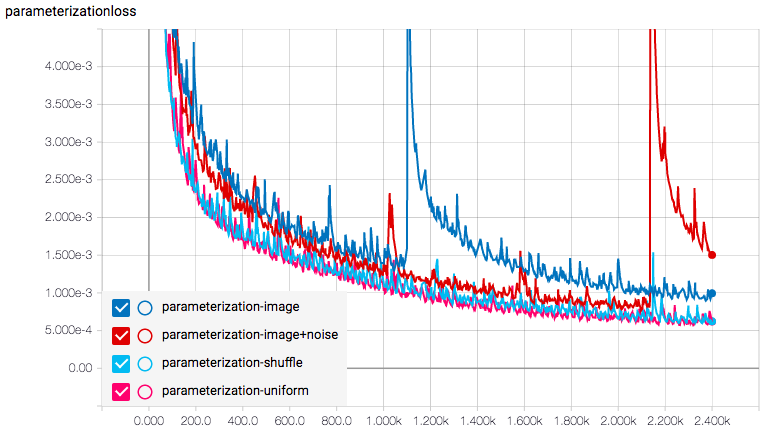
\includegraphics[width=0.8\textwidth]{parameterization.png}
\caption{\label{fig:parameterization} Parameterization loss curve.}
\end{figure}
\subsection{Denoising}
\begin{figure}[H]
\begin{tabular}{cc}
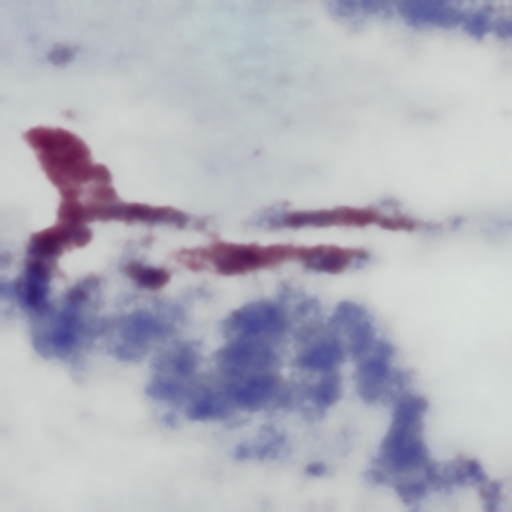
\includegraphics[width=80mm]{denoising-iteration-100.png} & 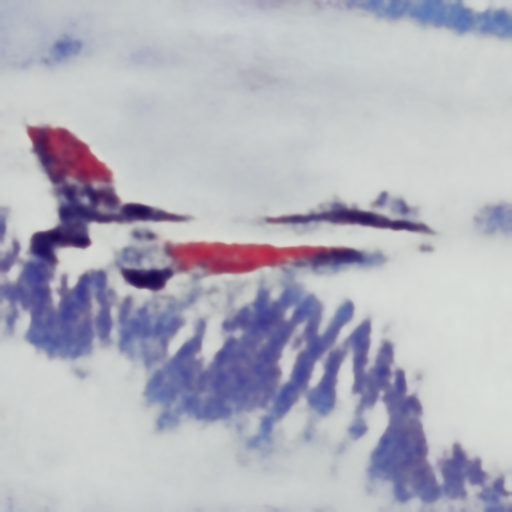
\includegraphics[width=80mm]{denoising-iteration-200.png} \\
(a) Denoising iteration 100 & (b) Denoising iteration 200 \\[6pt]
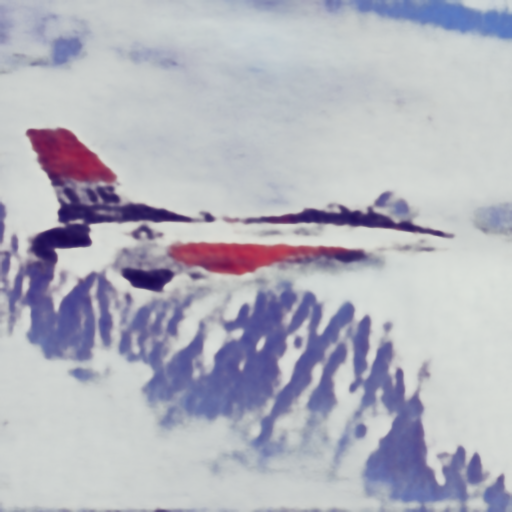
\includegraphics[width=80mm]{denoising-iteration-300.png} & 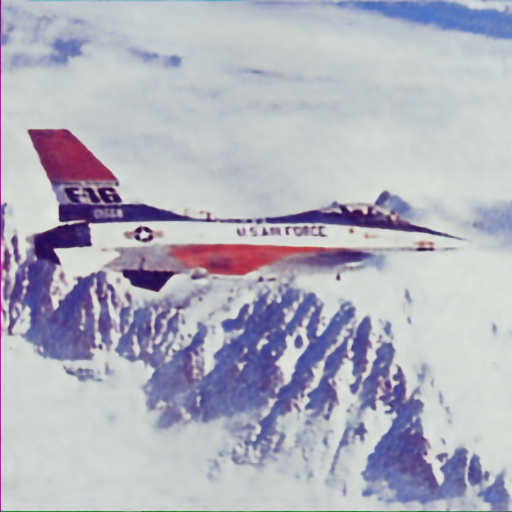
\includegraphics[width=80mm]{denoising-iteration-1800.png} \\
(c) Denoising iteration 300 & (d) Denoising iteration 1800 \\[6pt]
\multicolumn{2}{c}{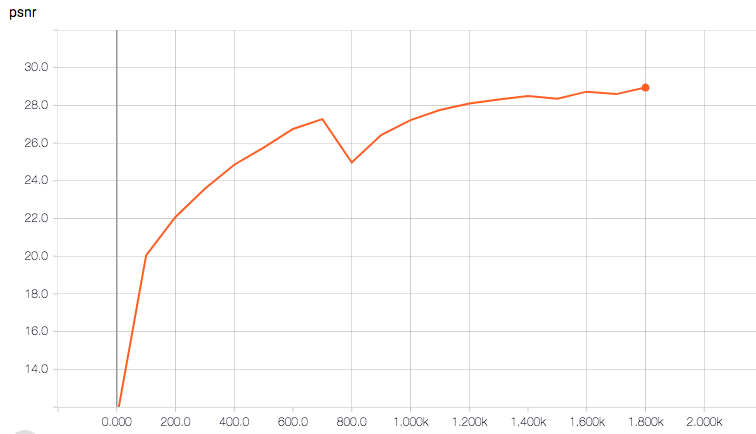
\includegraphics[width=80mm]{denoising-psnr.png}}\\
\multicolumn{2}{c}{(e) Denoising PSNR }
\end{tabular}
\caption{(a)(b)(c)(d) Shows the progress of denoising. (e) Final PSNR: 28.95}
\end{figure}
\subsection{Super Resolution}
\begin{figure}[H]
\begin{tabular}{cc}
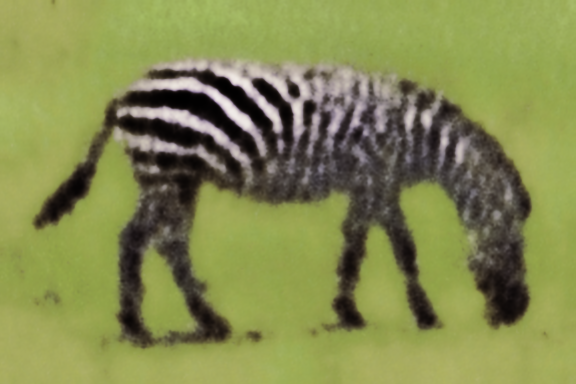
\includegraphics[width=80mm]{sr-iteration-100.png} & 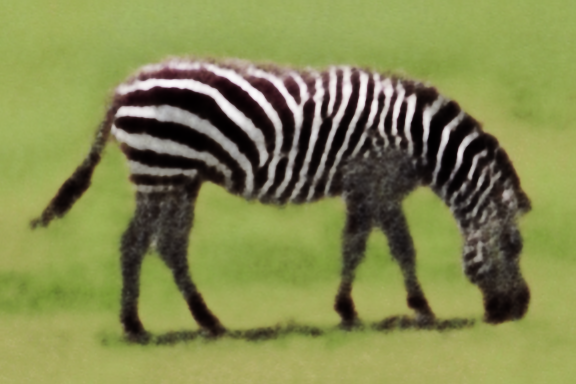
\includegraphics[width=80mm]{sr-iteration-200.png} \\
(a) Super-resolution iteration 100 & (b) Super-resolution 200 \\[6pt]
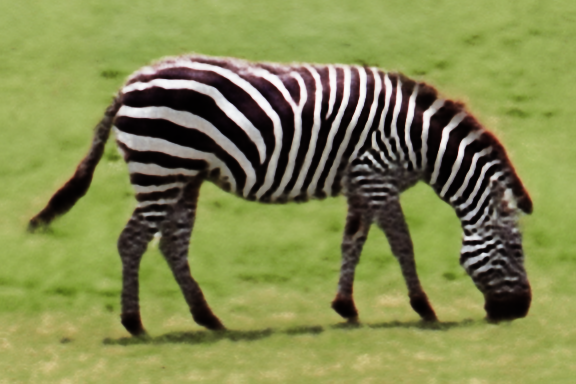
\includegraphics[width=80mm]{sr-iteration-400.png} & 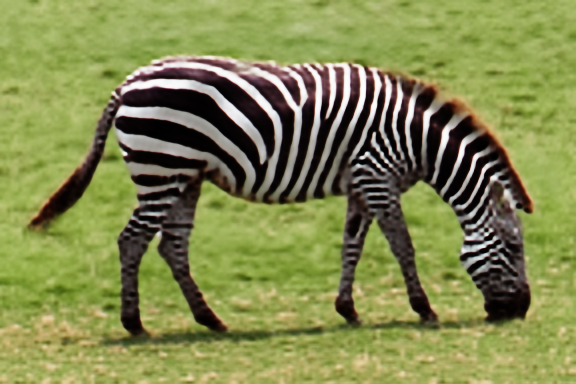
\includegraphics[width=80mm]{sr-iteration-2000.png} \\
(c) Super-resolution 400 & (d) Super-resolution 2000 \\[6pt]
\multicolumn{2}{c}{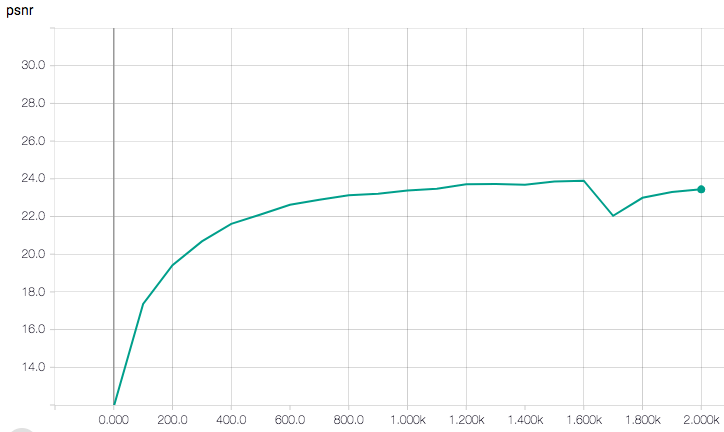
\includegraphics[width=80mm]{sr-psnr.png}}\\
\multicolumn{2}{c}{(e) Super-resolution PSNR }
\end{tabular}
\caption{(a)(b)(c)(d) Shows the progress of Super-resolution. (e) Final PSNR: 23.44}
\end{figure}
\subsection{Bonus Inpainting}
\begin{figure}[H]
\begin{tabular}{cc}

\includegraphics[width=80mm]{inpainting-iteration-100.png} & 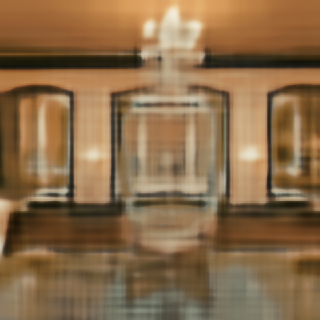
\includegraphics[width=80mm]{inpainting-iteration-200.png} \\
(a) Inpainting iteration 100 & (b) Inpainting 200 \\[6pt]
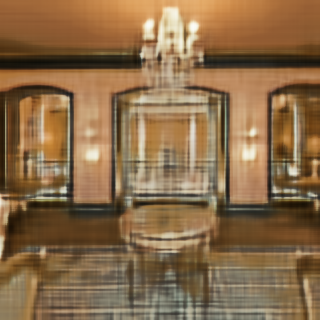
\includegraphics[width=80mm]{inpainting-iteration-300.png} & 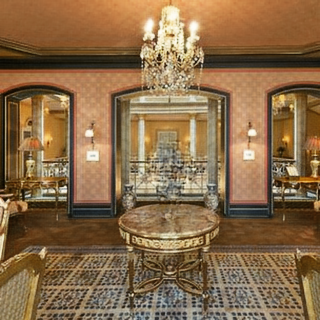
\includegraphics[width=80mm]{inpainting-iteration-5000.png} \\
(c) Inpainting 300 & (d) Inpainting 5000 \\[6pt]
\end{tabular}
\caption{(a)(b)(c)(d) Shows the progress of Inpainting}
\end{figure}
\section{Discussion}
For denoising, super-resolution and inpainting, the results are as expected.
However the result of parameterization is different from the original paper.
The speed of convergence is completely reversed.
Use uniform random noise as input converges the fastest.
And all the losses drop really quick at the beginning.
We didn't observe that uniform and shuffle suffer from slow convergence.
Maybe there are differences but the convergence is too fast.
So we didn't see the distinct difference of loss drop.

\begin{appendices}
\chapter{Source code for experiments}\\
\url{https://github.com/jxcodetw/NCTU_DeepLearning/tree/master/lab2}
\end{appendices}
\begin{figure}[H]
\begin{tabular}{cc}
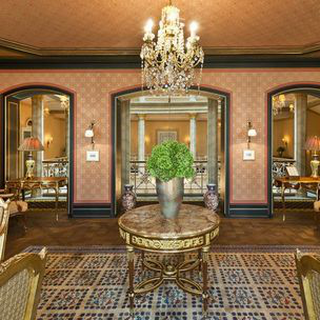
\includegraphics[width=80mm]{inpainting-gt.png} & 
\includegraphics[width=80mm]{inpainting-mask.png} \\
(a) Inpainting target & (b) Inpainting Mask \\[6pt]
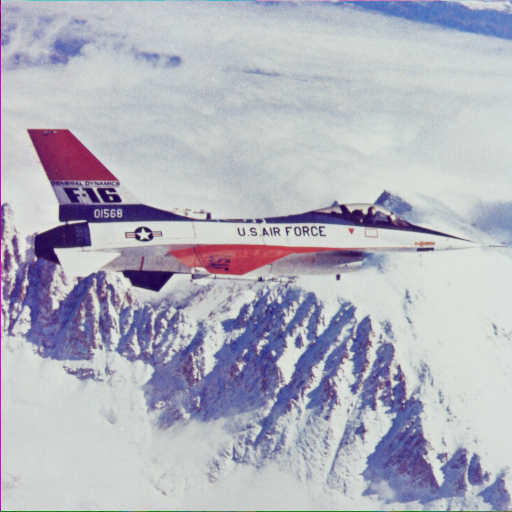
\includegraphics[width=80mm]{denoising-gt.png} & 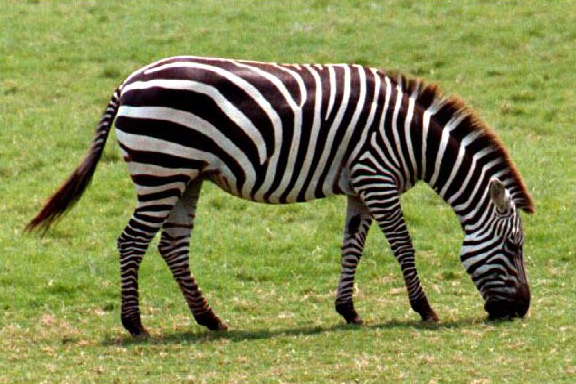
\includegraphics[width=80mm]{sr-gt.png} \\
(c) Denoising Ground Truth & (d) Super-resolution Ground Truth \\[6pt]
\multicolumn{2}{c}{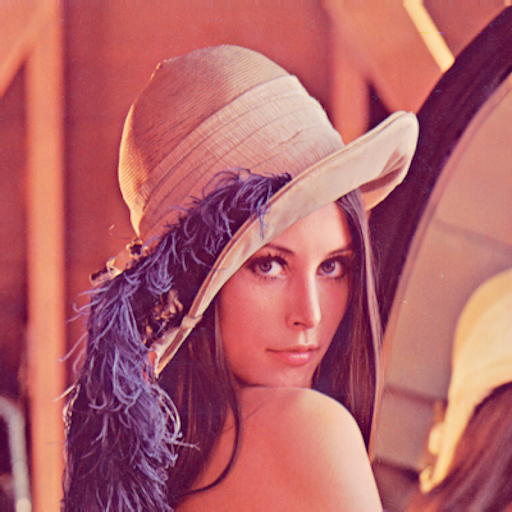
\includegraphics[width=80mm]{test-image.png}}\\
\multicolumn{2}{c}{(e) Parameterization }
\end{tabular}
\caption{(a)(b)(c)(d) The images we use as benchmark.}
\end{figure}
\end{document}